\section{重ね合わせの原理のみに依存する命題}

\begin{description}
\item[1.~定理.] \emph{一つの直線が別の直線と出会うとき、できる隣り合う角の和は二直角に等しい。}

\item[2.~定理.] \emph{二直線が交わるとき、対頂角は等しい。}

\item[3.~定理.] \emph{二つの三角形において、一方の一辺とその両端の角、または二辺とその間の角が、他方の対応する部分にそれぞれ等しければ、二つの三角形は等しい。}

\item[4.~定理.] \emph{二等辺三角形では、等しい辺に対する角は等しい。}

頂角を二等分し、(3) を用いる。

\item[5.~定理.] \emph{三角形の各辺の中点に立てた垂線のうち二本が交わるならば、三本は一点で交わり、この点は三角形の三つの頂点を通る円の中心である。}

\begin{figure}[h]
\centering
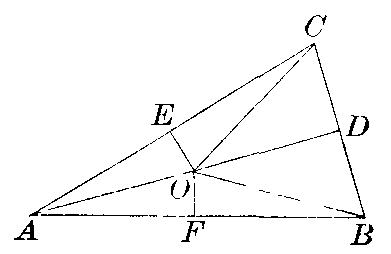
\includegraphics[width=40mm]{fig01.png}
\end{figure}

\textbf{証明.} $EO$ と $FO$ が $O$ で交わるとする。三角形 $AFO$ と $BFO$ は (3) により等しい。また $AEO$ と $CEO$ も等しい。したがって $CO$ と $BO$ は、ともに $AO$ に等しいから、等しい。ゆえに三角形 $BCO$ は二等辺三角形であり、角 $BOC$ を二等分するように引いた $OD$ は、$BC$ に対してその中点で垂直になる。

\item[6.~定理.] \emph{円において、中心での角を二等分する半径は、その角に対する弦に垂直であり、この弦を二等分する。}

\item[7.~定理.] \emph{円の中心における角は、切り取られる弧に比例し、弧によって測ることができる。}

\item[8.~定理.] \emph{直線外の任意の点から、その直線へ垂線を引くことができる。}

\begin{figure}[h]
\centering
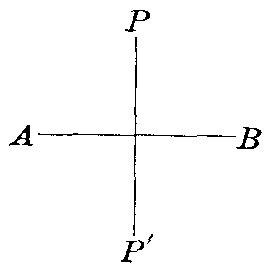
\includegraphics[width=20mm]{fig02.png}
\end{figure}

\textbf{証明.} 平面を $AB$ のまわりに回転させて自分自身に重ね合わせたとき、点 $P$ が移る位置を $P'$ とする。そのとき、直線 $PP'$ は $AB$ に垂直である。

\item[9.~定理.] \emph{直線に立てた垂線上の一点から斜線を引き、垂線の足から等しい距離のところを切り取るならば、それらの斜線は等しく、直線となす角も垂線となす角も等しい。}

\begin{figure}[h]
\centering
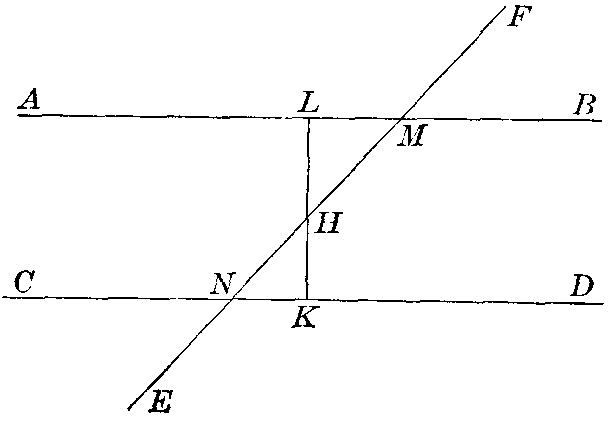
\includegraphics[width=50mm]{fig03.png}
\end{figure}

\item[10.~定理.] \emph{二直線が第三の直線と同じ角で交わる、すなわち対応する角が等しいならば、その二直線の両方に垂直な直線を引くことができる。}

\textbf{証明.} 角 $FMB$ と $MND$ が等しいとし、$MN$ の中点 $H$ を通って $CD$ に垂直に $LK$ を引く。このとき $LK$ は $AB$ にも垂直である。なぜなら、二つの三角形 $LMH$ と $KNH$ が (3) により等しいからである。

\item[11.~定理.] \emph{平面上で、与えられた直線に垂直に立てた等しい二本の線分があるとき、それらの端点を結ぶ線は二本の線分と等しい角をなし、両者の中間に立てた第三の垂線によって、直角に二等分される。}

\begin{figure}[h]
\centering
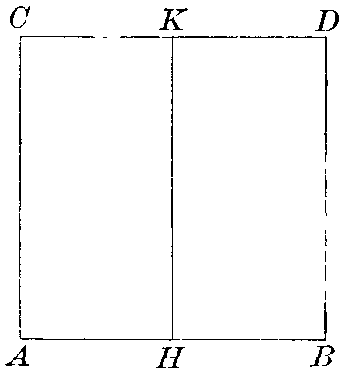
\includegraphics[width=40mm]{fig04.png}
\end{figure}

\textbf{$AC$ と $BD$} が $AB$ に垂直で、$AC$ と $BD$ が等しいとする。$C$ と $D$ を結ぶ線が $C$ と $D$ でなす角は等しく、$AB$ の中点に立てた垂線 $HK$ は、$CD$ に対してその中点で垂直である。

重ね合わせにより証明される。

\item[12.~定理.] \emph{前の命題のように二本の垂線と、その中間に立てた第三の垂線が与えられているとき、この第三の垂線に直角に交わる任意の直線は、最初の二本と交わるならば、それらの上に等しい長さを切り取り、等しい角をなす。}

重ね合わせにより証明される。

\begin{figure}[h]
\centering
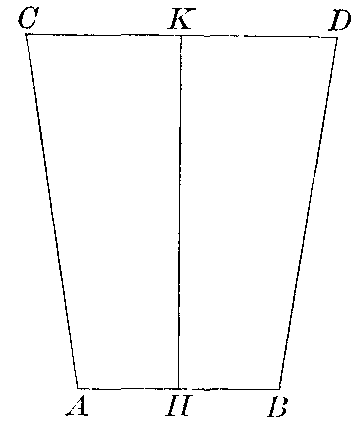
\includegraphics[width=40mm]{fig05.png}
\end{figure}

\textbf{系.} \emph{前の二つの命題は、$A$ と $B$ での角が等しい鋭角、または等しい鈍角であって、$HK$ が $AB$ の中点で $AB$ に垂直である場合にも成り立つ。$AC = BD$ ならば、$C$ と $D$ での角は等しく、$HK$ は $CD$ に対してその中点で垂直である。または、$CD$ が $HK$ に任意の点 $K$ で垂直であり、$AC$ と $BD$ と交わるならば、それはこの二直線上に等しい距離を切り取り、等しい角をなす。}
\end{description}

\section{限定された図形について成り立つ命題}

つぎの命題は、少なくとも、線の長さがある一定の長さを超えない図形について成り立つ。すなわち、例外があるとしても、それは線のどこかの長さのために、定理あるいは証明のある段階を適用できないような場合にあたる。便宜上、この意味で\emph{限定された}という語を用い、ある定理が限定された図形について、あるいは平面の限定された部分において成り立つ、と言うことにする。

\begin{figure}[h]
\centering
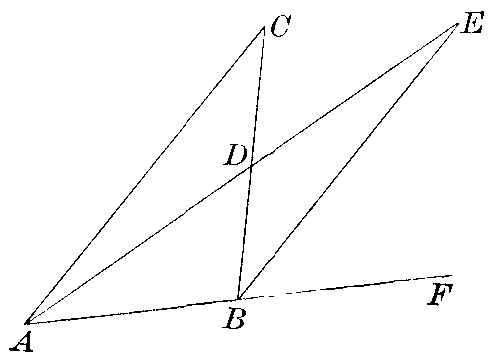
\includegraphics[width=40mm]{fig06.png}
\end{figure}

\begin{description}
\item[1.~定理.] \emph{三角形の外角は、それに隣り合わない内角のどちらよりも大きい}（ユークリッド、I, 16）。

\textbf{証明.} $A$ から対辺の中点まで $AD$ を引き、それを延長して $DE = AD$ となるように $E$ をとる。二つの三角形 $ADC$ と $EBD$ は等しく、角 $FBD$ は角 $EBD$ より大きいから、$C$ より大きい。

\textbf{系.} \emph{三角形の少なくとも二つの角は鋭角である。}

\item[2.~定理.] \emph{三角形の二つの角が等しければ、それに対する辺は等しく、その三角形は二等辺三角形である。}

\begin{figure}[h]
\centering
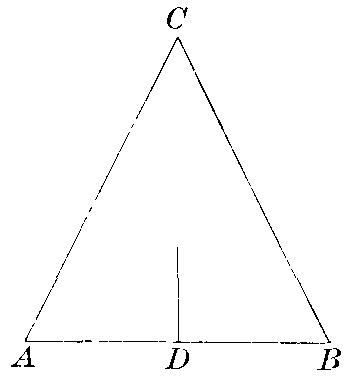
\includegraphics[width=40mm]{fig07.png}
\end{figure}

\textbf{証明.} 底辺の中点に立てた垂線は、三角形を、互いに重ね合わせることができて等しい二つの図形に分ける。したがってこの垂線は頂点を通り、等しい角に対する二辺は等しい。

\item[3.~定理.] \emph{角が等しくない三角形では、大きいほうの角に対する辺は、小さいほうの角に対する辺より大きい。逆に、三角形の辺が等しくなければ、対する角も等しくなく、大きい角は大きい辺に対する。}

\item[4.~定理.] \emph{二つの三角形において、一方の二辺が他方の二辺にそれぞれ等しく、しかも第一の三角形の挟む角が第二の三角形の挟む角より大きいならば、第一の三角形の第三辺は第二の三角形の第三辺より大きい。逆に、二つの三角形において、一方の二辺が他方の二辺にそれぞれ等しく、しかも第一の三角形の第三辺が第二の三角形の第三辺より大きいならば、第一の三角形の第三辺に対する角は、第二の三角形の第三辺に対する角より大きい。}

\item[5.~定理.] \emph{任意の点から直線の両端へ引いた二線の和は、同様に引いてそれらに囲まれた二線の和より大きい。}

\item[6.~定理.] \emph{一点を通って直線へ引ける垂線は、ただ一本である。}

\begin{figure}[h]
\centering
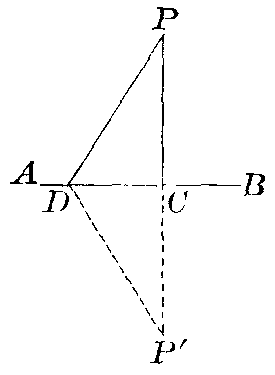
\includegraphics[width=30mm]{fig08.png}
\end{figure}

\textbf{証明.} 平面を $AB$ のまわりに回転させて自分自身に重ね合わせたとき、点 $P$ が移る位置を $P'$ とする。$P$ から $AB$ へ二本の垂線 $PC$ と $PD$ が引けるとすると、$CP'$ と $DP'$ はこれらの線の延長となり、$P$ と $P'$ を結ぶ異なる二本の直線ができることになるが、それは不可能である。

\textbf{系.} \emph{二つの直角三角形は、一方の斜辺と一つの鋭角が、他方の斜辺と一つの鋭角にそれぞれ等しいとき、等しい。}

\item[7.~定理.] \emph{垂線は、点から直線へ引くことのできる線のうちで最も短い。}

\textbf{系.} \emph{直角三角形では、斜辺は、直角をはさむ二辺のどちらよりも大きい。}

\item[8.~定理.] \emph{直線に立てた垂線上の一点から斜線を引き、垂線の足から等しくない距離のところを切り取るならば、それらの斜線は等しくなく、遠いほうが大きい。逆に、垂線上の一点から引いた二本の斜線が等しくなければ、大きいほうが垂線の足からより大きい距離を切り取る。}

\item[9.~定理.] \emph{線分の中点に垂線を立てたとき、その垂線上にない任意の点は、垂線に関して同じ側にある線分の端点により近い。}

\textbf{系.} \emph{線分の両端から等距離にある二点は、その線分にその中点で垂直な直線を決定する。}

\item[10.~定理.] \emph{二つの三角形は、一方の三辺が他方の三辺にそれぞれ等しいとき、等しい。}

\item[11.~定理.] \emph{平面上で、第三の直線に垂直に立てた二本の線が等しくなければ、それらの端点を結ぶ線が二本の線となす角も等しくなく、短い垂線とのなす角のほうが大きい。}

\begin{figure}[h]
\centering
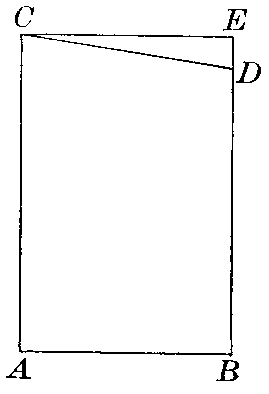
\includegraphics[width=25mm]{fig09.png}
\end{figure}

\textbf{証明.} $AC > BD$ とする。$BD$ を延長して $BE = AC$ とする。すると $BEC = ACE$ である。しかし (1) により $BDC > BEC$ であり、$ACD$ は $ACE$ の一部である。したがって、なおさら $BDC > ACD$ である。

\item[12.~定理.] \emph{$C$ と $D$ での二つの角が等しければ、垂線は等しく、角が等しくなければ、垂線も等しくなく、長いほうの垂線は小さいほうの角をなす。}

\item[13.~定理.] \emph{二直線が第三の直線に垂直であるとき、一方の直線上の点で第三の直線から等距離にあるものは、他方の直線からも等距離にある。}

\begin{figure}[h]
\centering
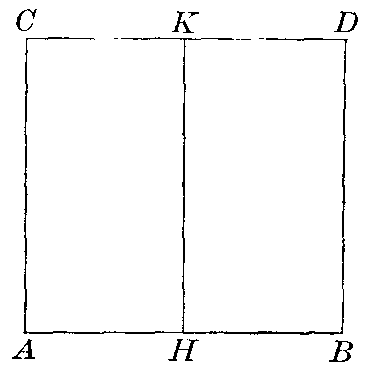
\includegraphics[width=30mm]{fig10.png}
\end{figure}

\textbf{証明.} $AB$ と $CD$ が $HK$ に垂直であるとし、$CD$ 上に $K$ から等距離にある任意の二点 $C$ と $D$ をとる。すると $C$ と $D$ は $AB$ から等距離にある。なぜなら、重ね合わせにより $D$ を $C$ に重ねることができ、そのとき (6) により $DB$ は $CA$ に重なるからである。
\end{description}

\medskip 立体幾何学のつぎの命題は、直接に前の諸命題に依存し、少なくとも空間の任意の限定された部分で成り立つ。

\begin{description}
\item[14.~定理.] \emph{一直線が、交わる二直線にその交点で垂直ならば、それは、その交点を通る二直線の平面上のすべての直線に垂直である。}

\item[15.~定理.] \emph{二つの平面が垂直ならば、一方の平面内でそれらの交線に垂直に引いた直線は、他方の平面に垂直である。また、一方の平面の任意の点を通って他方の平面に垂直に引いた直線は、完全に前者の平面内にある。}

\item[16.~定理.] \emph{直線が平面に垂直ならば、その直線を通る任意の平面は、その平面に垂直である。}

\item[17.~定理.] \emph{平面が、交わる二つの平面のそれぞれに垂直ならば、その平面はそれらの交線に垂直である。}
\end{description}

\section{三つの仮説}

二本の等しい垂線の端点での角は、少なくとも限定された図形については、直角か、鋭角か、鈍角のいずれかである。この三つの場合を、それぞれ\emph{直角の仮説}、\emph{鋭角の仮説}、\emph{鈍角の仮説}と呼んで区別する。

\begin{description}
\item[1.~定理.] \emph{二本の等しい垂線の端点を結ぶ線は、少なくとも平面の任意の限定された部分では、三つの仮説に応じて、それぞれ垂線の足を結ぶ線に等しいか、より大きいか、より小さい。}

\begin{figure}[h]
\centering
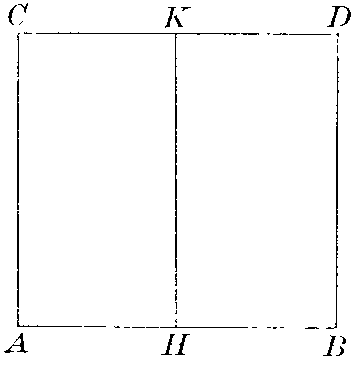
\includegraphics[width=35mm]{fig11.png}
\end{figure}

\textbf{証明.} $AC$ と $BD$ を二本の等しい垂線とし、$HK$ を $AB$ の中点に立てた第三の垂線とする。このとき $HA$ と $KC$ は $HK$ に垂直であり、$C$ での角が $A$ での角に等しいか、より小さいか、より大きいかに応じて、$KC$ は $HA$ に等しいか、より大きいか、より小さい（II, 12）。したがって、$KC$ の二倍である $CD$ は、三つの仮説に応じて、それぞれ $AB$ に等しいか、より大きいか、より小さい。

\textbf{逆に、}$CD$ が $AB$ に等しいか、より大きいか、より小さいと与えられるならば、この図形について、それぞれ第一、第二、第三の仮説が成り立つ。

\textbf{系.} \emph{四角形が三つの直角をもつとき、第四の角に隣り合う辺は、第四の角が直角か、鋭角か、鈍角かに応じて、それぞれの対辺に等しいか、より大きいか、より小さい。}

\item[2.~定理.] \emph{直角の仮説が、平面の任意の限定された部分における一つの場合に成り立つならば、それはあらゆる場合に、平面全体で成り立つ。}

\begin{figure}[h]
\centering
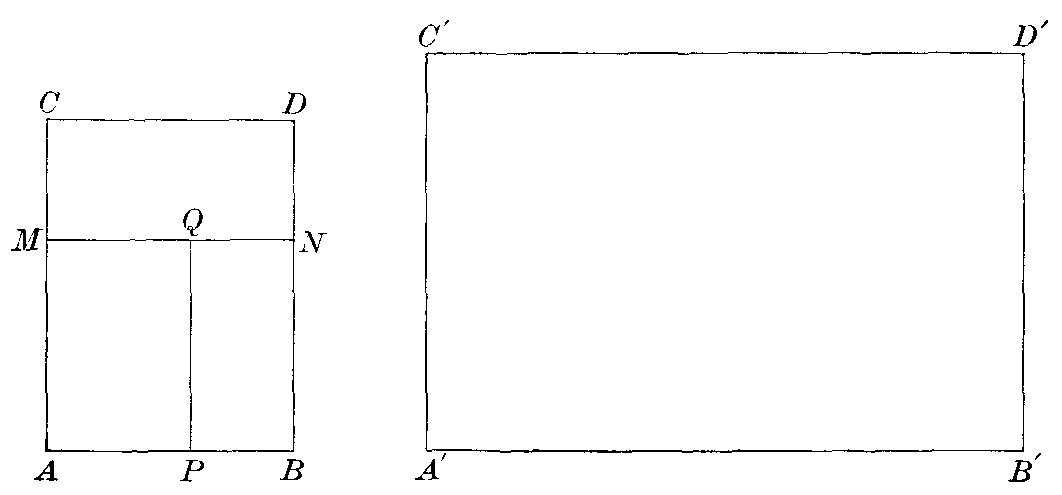
\includegraphics[width=75mm]{fig12.png}
\end{figure}

\textbf{証明.} ここでは長方形、すなわち四つの角がすべて直角の四角形がある。前の命題の系により、その対辺は等しい。等しい長方形は、辺が与えられた長方形の対応する辺の任意の倍数となるような長方形をつくるように、並べて置くことができる。

さて、$A'B'$ を任意の線分とし、$A'C'$ と $B'D'$ をその両端で $A'B'$ に垂直な等しい二線とする。$A'C'$ を、必要ならばいくつかの等しい部分に分けて、その一つが $AC$ より小さくなるようにし、$AC$ と $BD$ の上に、そのうちの一つに等しい $AM$ と $BN$ をとり、$MN$ を引く。$ABNM$ は長方形である。そうでなければ、$MN$ は $AB$ と $CD$ より大きいか小さいかであり、$M$ と $N$ での角はすべて鋭角か、すべて鈍角になるが、それらの和はちょうど四直角であるから、これは不可能である。つぎに、$A'B'$ を十分な個数の等しい部分に分け、その一つを $AB$ と $MN$ 上にとり、長方形 $APQM$ をつくる。これに等しい長方形を並べて、図形 $A'B'D'C'$ をちょうど覆うことができるから、この図形自身も長方形でなければならない。

\item[3.~定理.] \emph{鋭角の仮説または鈍角の仮説が、平面の限定された部分内の一つの場合に成り立つならば、同じ仮説が、平面のそのような任意の部分内のあらゆる場合に成り立つ。}

\begin{figure}[h]
\centering
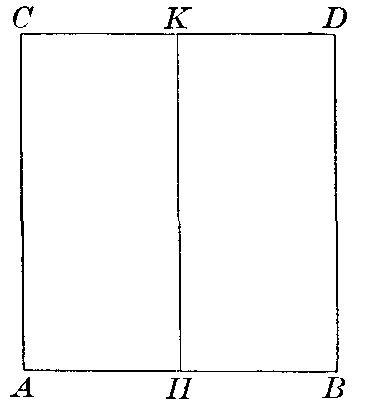
\includegraphics[width=35mm]{fig13.png}
\end{figure}

\textbf{証明.} $CD$ を $AC$ と $BD$ に沿って動かし、この二線上に常に等しい距離を切り取るようにする。あるいはまた、$AC$ と $BD$ を線 $AB$ に沿って $HK$ のほうへ、または $HK$ から遠ざかるように動かし、つねに $AB$ に垂直であって、その足が $H$ から常に等距離にあるようにする。$C$ と $D$ での角は連続的に変化するから、鋭角あるいは鈍角のままでいるか、あるいはどこかで直角になるかのいずれかでなければならない。直角になるとすれば、直角の仮説が成り立つことになり、仮定した一つの場合においてすら、鋭角の仮説も鈍角の仮説も成り立ち得ない。

$C$ と $D$ での角は、平面の限定された部分では、零にも $180^\circ$ にもなり得ない。なぜなら、そうなれば三つの線 $AC$、$CD$、$BD$ が同一の直線になってしまうからである。

\item[4.~定理.] \emph{三角形の内角の和は、少なくとも平面の任意の限定された部分では、三つの仮説に応じて、それぞれ二直角に等しいか、より小さいか、より大きい。}

\begin{figure}[h]
\centering
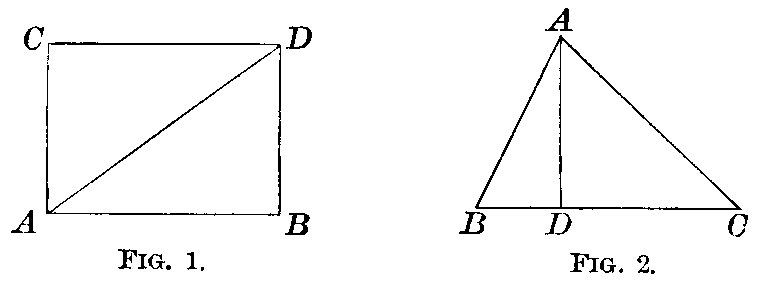
\includegraphics[width=80mm]{fig14.png}
\end{figure}

\textbf{証明.} $B$ に直角をもつ任意の三角形 $ABD$（図1）が与えられたとして、$AB$ に垂直に、$BD$ に等しい $AC$ を引く。三角形 $ADC$ と $DAB$ において、$AC=BD$ で $AD$ は共通であるが、$DC$ は三つの仮説に応じて、それぞれ $AB$ に等しいか、より大きいか、より小さい。したがって、$DAC$ は三つの仮説に応じて、それぞれ $ADB$ に等しいか、より大きいか、より小さい（II, 4）。この二つの角のそれぞれに $BAD$ を加えると、$ADB + BAD$ は直角 $BAC$ に等しいか、それより小さいか、それより大きいことになる。

さて、限定された任意の三角形の少なくとも二つの角は鋭角である。したがって、第三の角の頂点から対辺へ下ろした垂線は、その辺と三角形の内部で出会い、三角形を二つの直角三角形に分ける。ゆえに、限定された任意の三角形において、角の和は三つの仮説に応じて、それぞれ二直角に等しいか、より小さいか、より大きい。

三角形の角の和が二直角を超える量を、その\emph{過剰}と呼ぶ。$n$ 辺の多角形の過剰とは、その角の和が二直角の $n-2$ 倍を超える量である。

辺上の任意個の点を付加的な頂点と数えても、過剰は変わらない。このとき角の和には、そのような点ごとに二直角が加わるからである。

\item[5.~定理.] \emph{多角形の過剰は、それを分割してできる三角形の任意の系の過剰の和に等しい。}

\begin{figure}[h]
\centering
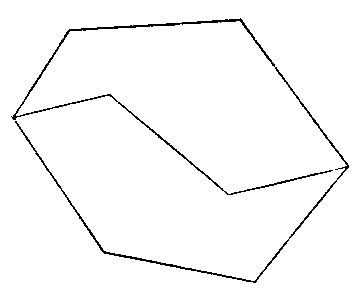
\includegraphics[width=30mm]{fig15.png}
\end{figure}

\textbf{証明.} 多角形を直線または折れ線で二つの多角形に分けるとき、その線が境界と出会う二点は頂点であるとしてよい。分割する線が $p$ 個の点で折れる折れ線であるならば、二つの多角形の辺は、もとの多角形の辺と、分割線が $p$ 個の点で分けられてできる $p+1$ 個の部分（それぞれ二度ずつ数える）とからなる。

もとの多角形の角の和を $S$、辺の数を $n$ とする。それが分けられてできた二つの多角形について、$S'$ と $n'$、$S''$ と $n''$ は同じ意味をもつとする。直角を $R$ と書くと、
\begin{align*}
S' + S'' &= S + 4pR, \\
\intertext{および}
n' + n'' &= n + 2(p+1). \\
\intertext{したがって、}
S' - 2(n'-2)R + S'' - 2(n''-2)R &= S + 4pR - 2(n+2p-2)R \\
&= S-2(n-2)R.
\end{align*}

多角形を分割してできる三角形の任意の系は、以上の過程を十分な回数くり返すことによって得られる。多角形の過剰は、つねに、それを分割してできる部分の過剰の和に等しい。

過剰の概念を拡張して、完全に直線で囲まれた平面の異なる部分の、任意の組み合わせに適用することもできる。

多角形の角の和を考える代わりに、外角の和をとってもよい。この和が四直角に足りない量は、多角形の過剰に等しい。これを外角の\emph{不足}ということができる。

\begin{figure}[h]
\centering
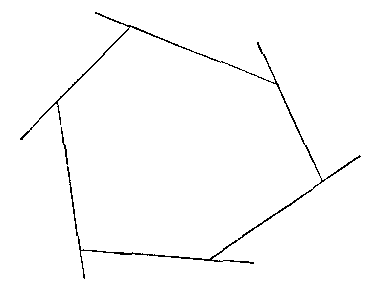
\includegraphics[width=30mm]{fig16.png}
\end{figure}

外角の和は、図形のまわりをちょうど一周するとき、各頂点で一つの辺から次の辺へ向きを変える、その回転量である。二つ以上の多角形の組み合わせを考えるときは、考える領域がつねに一方の側、たとえば左側にあるように、境界全体をたどらなければならない。

\item[6.~定理.] \emph{多角形の過剰は、つねに零であるか、つねに負であるか、つねに正である。}

\textbf{証明.} この定理が、限定された三角形について成り立つことはわかっている。しかし、有限な多角形は、有限個のそのような三角形に分割できるから、前の定理により、多角形の過剰はそれらの三角形の過剰の和に等しい。

過剰が負であるときは、それを不足と呼ぶか、外角の過剰と言うことができる。

\textbf{系.} \emph{多角形の過剰は、直線によってそれから切り取られる任意の部分の過剰より、数値として大きい。ただし第一の仮説では零である。}
\end{description}

\medskip つぎの定理は、第二および第三の仮説に適用される。

